\section{Concentração da frota}

A proposta deste estudo é evidenciar, através de um mapa de calor, onde estão concentrados os ônibus pela cidade ao longo de um dia. Pode ser usada como ferramenta para o planejamento de novas linhas e redistribuição das atuais. 

Apesar de ser difícil extrair conclusões apenas com este mapa, ele pode servir como uma ferramenta visual para observar em que vias e regiões da cidade estão concentrados os ônibus. Um exemplo é a figura \ref{fig:LABEL_FIG_ANALISE_CONCENTRACAO_CIDADE}, que traz uma visão geral da cidade do Rio de Janeiro.

\begin{figure}
  \centering
  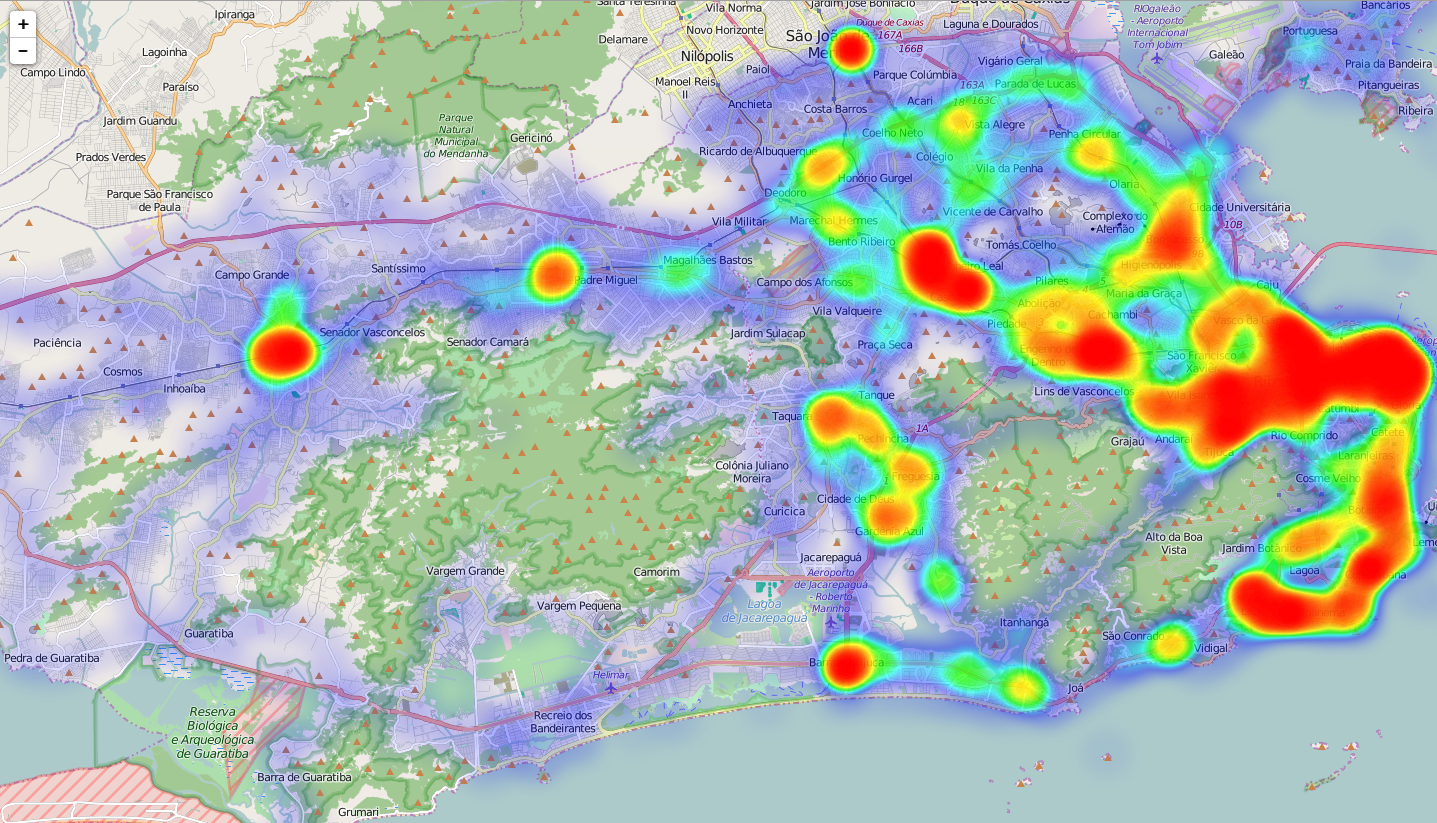
\includegraphics[width=1.0\textwidth]{imagens/heat_map1.png}
  \caption{Vista geral da cidade mostra uma grande concentração de ônibus nas regiões centrais. (Outubro de 2015)}
  \label{fig:LABEL_FIG_ANALISE_CONCENTRACAO_CIDADE}
\end{figure}


\subsection{Implementação}

Por ser uma análise mais simples, o esforço maior desta análise foi na parte da apresentação dos dados, ao invés da extração dos mesmos. 

Para extrair os dados, foi feita uma consulta no banco de dados por todos os registros geolocalizados em uma data específica. Como extrair e plotar esses dados diretamente seria muito demorado - há mais de 15 milhões de registros por dia - optamos por reduzir manualmente a precisão desses dados, agrupando registros muito próximos.

Para agrupar essas amostras, limitamos na nossa consulta a precisão dos campos de latitude e longitude de cada registro, utilizando uma precisão máxima de 4 casas decimais ao invés de 6. Só isso já reduz nosso número de amostras em cerca de 35 vezes, para cerca de 420.000 amostras, ainda mantendo uma boa precisão visual dos dados. 

Finalmente, a fim de descobrir quantos ônibus estavam em cada coordenada, foi utilizada a quantidade de registros naquela posição, contando apenas veículos distintos (cada ônibus é identificado por um número de ordem). Temos então como saída uma lista de coordenadas e suas respectivas quantidades de ônibus. 

Cada coordenada é plotada no gráfico através de uma escala de cores que representa a densidade de ônibus naquela região\cite{heatmap}. Como resultado, temos cores entre o azul escuro, que representa uma baixa densidade de ônibus na região, e o vermelho, que representa uma alta densidade. As escalas de cores foram normalizadas entre os estudos para preservar facilitar a comparação entre diferentes mapas.

Para a visualização desses dados, foi elaborada uma página que renderiza um mapa interativo, no qual é possível alterar a região de estudo e observar com maior precisão os resultados, permitindo focar em bairros ou ruas específicas. Quando duas amostras são comparadas, é possível visualizá-las lado-a-lado, atualizando simultaneamente conforme o mapa é movimentado pelo usuário.


\subsection{Resultados observados}

O mapa de calor se torna ainda mais útil quando são comparados dados de diferentes períodos, a fim de analisar como mudou a distribuição dos ônibus ao longo do tempo.

Uma das comparações feitas foi entre dados de dois anos consecutivos, 2015 e 2016. Foram analisados dados do mesmo dia, 8 de julho, um dia útil, nos dois anos. A comparação entre esses anos é especialmente relevante pois, desde o final de 2015 até a data atual, ocorrem grandes mudanças nas linhas de ônibus do Rio de Janeiro, em especial devido ao plano de racionalização das linhas da Zona Sul\cite{noticia_racionalizacao}. Além disso, devido a grandes obras pela cidade, houve diversas interdições no trajeto das linhas, a construção de novas vias e implantação de novos corredores exclusivos de ônibus.

Na figura \ref{fig:LABEL_FIG_ANALISE_RACIONALIZACAO}, é possível visualizar essa comparação e observar uma enorme diminuição dos ônibus nos bairros da Zona Sul próximos à Lagoa Rodrigo de Freitas. 

\begin{figure}
  \centering
  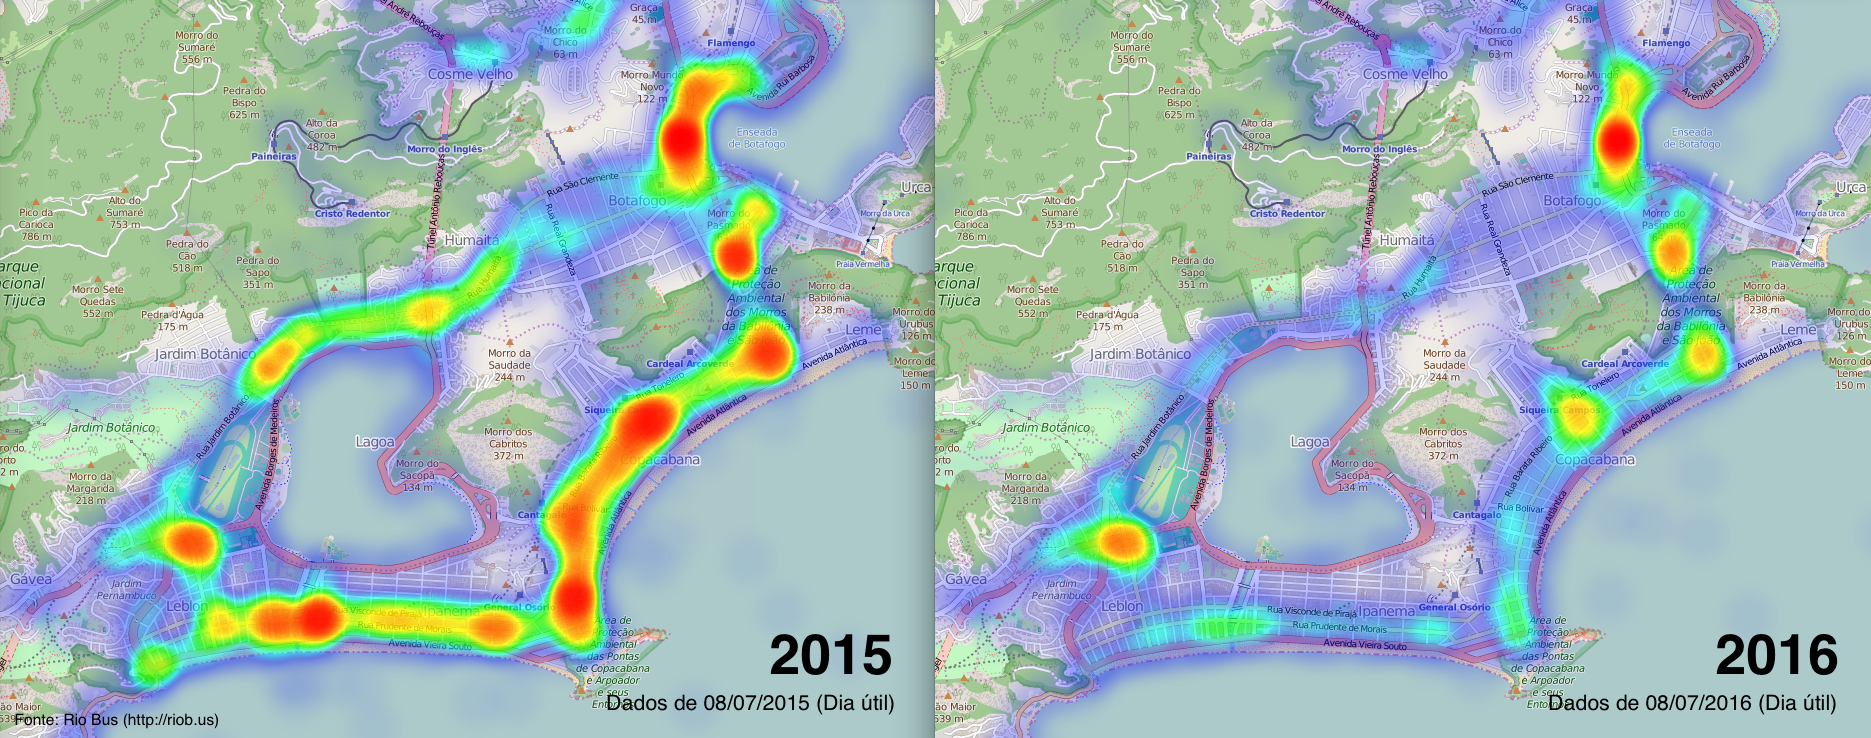
\includegraphics[width=1.0\textwidth]{imagens/heat_map_zs201516.png}
  \caption{Comparação da quantidade de ônibus na Zona Sul em dois anos consecutivos. Em 2016, observa-se a redução em virtude da racionalização das linhas de ônibus.}
  \label{fig:LABEL_FIG_ANALISE_RACIONALIZACAO}
\end{figure}


No Centro da cidade, observa-se através da figura \ref{fig:LABEL_FIG_ANALISE_CONCENTRACAO_CENTRO} que as principais vias da região concentram praticamente toda a circulação dos ônibus, enquanto vias transversais não possuem quase nenhum tráfego desse tipo.

\begin{figure}
  \centering
  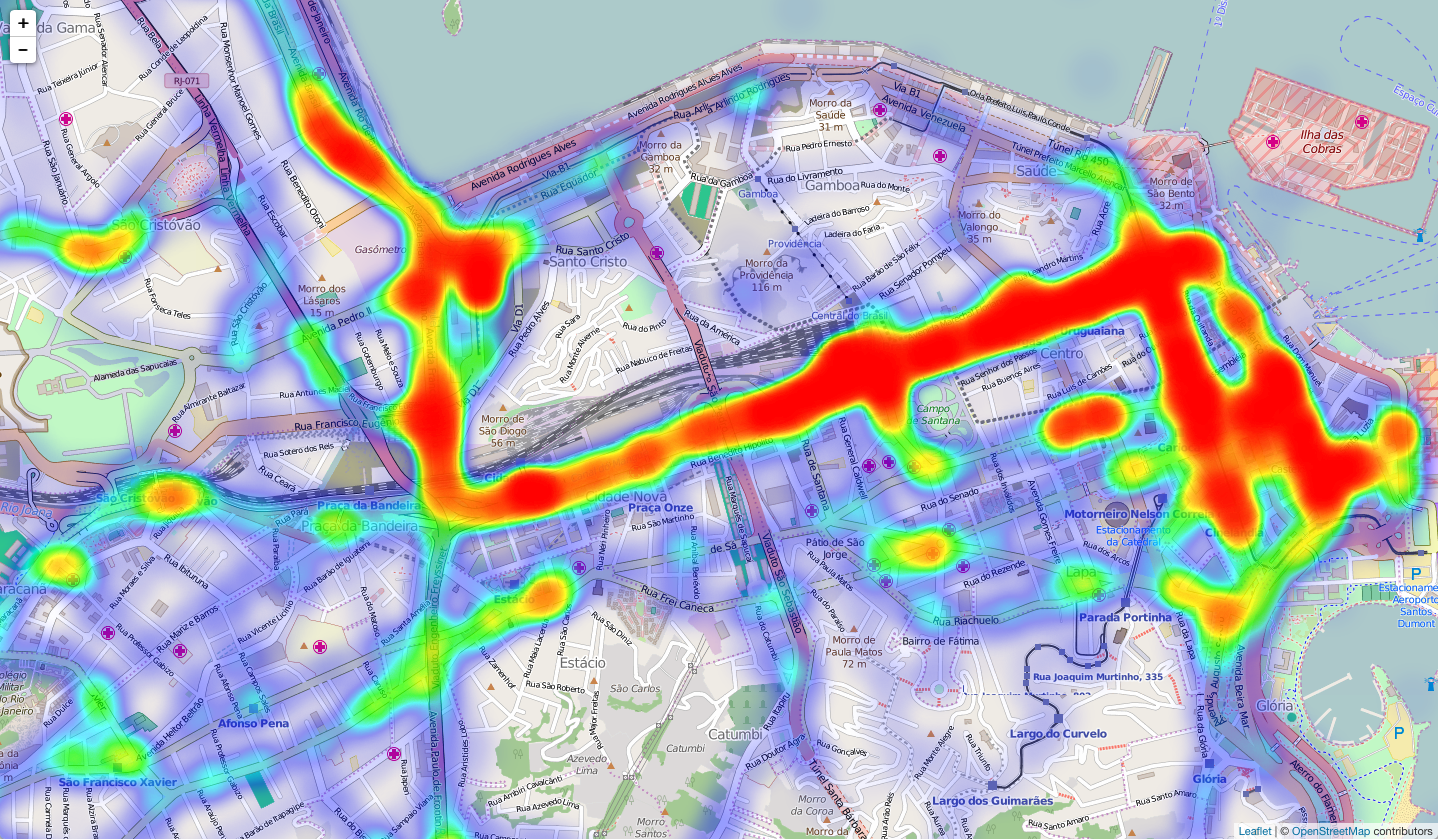
\includegraphics[width=0.9\textwidth]{imagens/heat_map2.png}
  \caption{No Centro, concentração alta nas vias principais e baixa nas transversais. (Outubro de 2015)}
  \label{fig:LABEL_FIG_ANALISE_CONCENTRACAO_CENTRO}
\end{figure}

% \begin{figure}
%   \centering
%   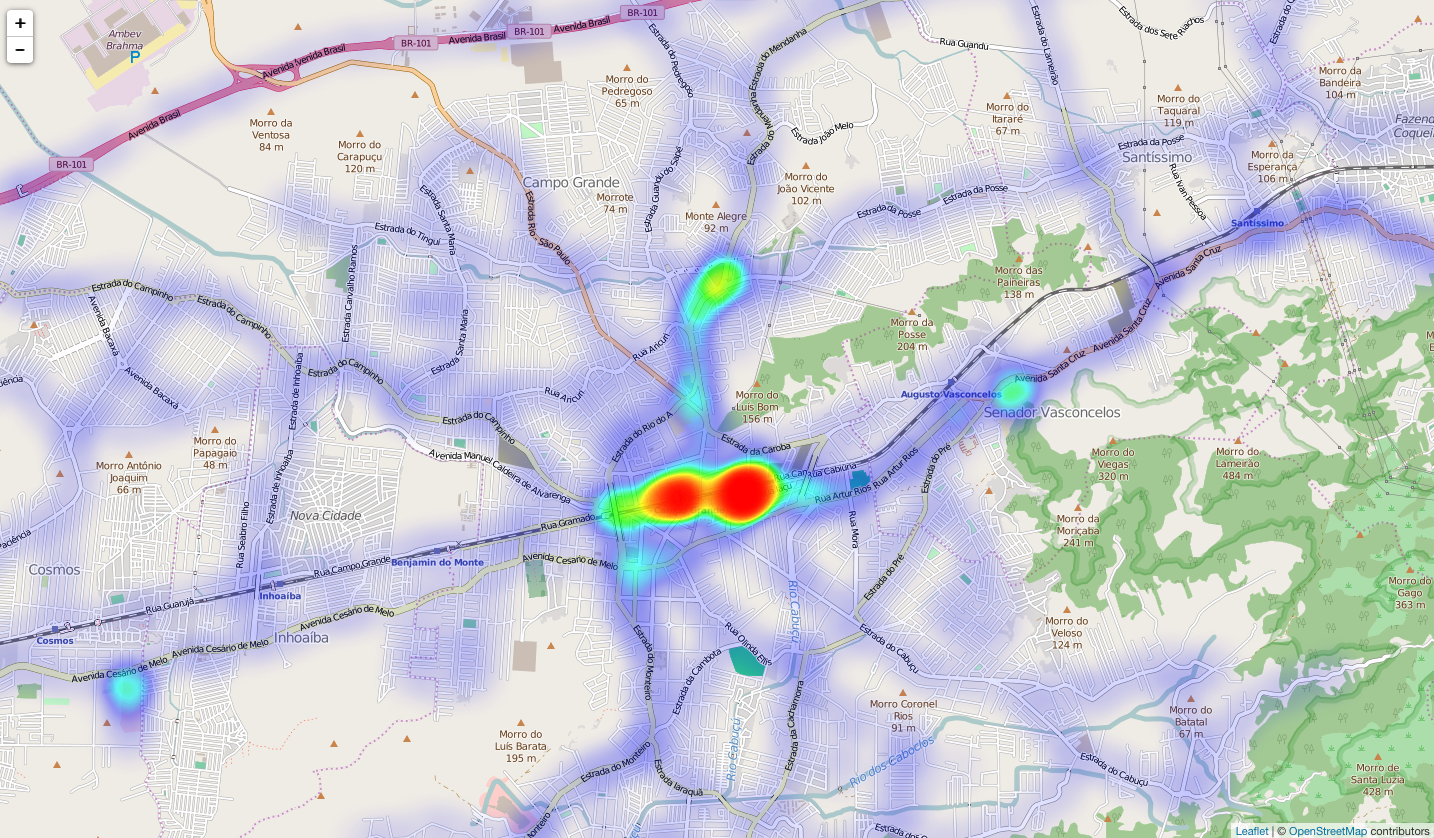
\includegraphics[width=1.0\textwidth]{imagens/heat_map3.png}
%   \caption{Enorme concentração em um único trecho em Campo Grande. (Outubro de 2015)}
%   \label{fig:LABEL_FIG_ANALISE_CONCENTRACAO_3}
% \end{figure}